%\documentclass[preprint,10pt,authoryear]{elsarticle}
\documentclass[preprint,10pt,authoryear]{article}

% amsmath package, useful for mathematical formulas
\usepackage{amsmath}
% amssymb package, useful for mathematical symbols
%\usepackage{amssymb}

% graphicx package, useful for including eps and pdf graphics
% include graphics with the command \includegraphics
\usepackage{graphicx}

% cite package, to clean up citations in the main text. Do not remove.
%\usepackage{cite}
\usepackage{natbib}

\usepackage{color} 

% Use doublespacing - comment out for single spacing
\usepackage{setspace} 
\doublespacing

% Use lscape packages to allow for specific pages to be displayed as landscape
% \usepackage{lscape}
\usepackage{pdflscape}

\usepackage{xr}
\externaldocument{chemokine_main_revised}


% Text layout
\topmargin 0.0cm
\oddsidemargin 0.5cm
\evensidemargin 0.5cm
\textwidth 16cm 
\textheight 21cm

% Bold the 'Figure #' in the caption and separate it with a period
% Captions will be left justified
\usepackage[labelfont=bf,labelsep=period,justification=raggedright]{caption}

\bibliographystyle{elsarticle-num-names}

% Remove brackets from numbering in List of References
\makeatletter
\renewcommand{\@biblabel}[1]{\quad#1.}
\makeatother


% Leave date blank
\date{}

\pagestyle{myheadings}
%% ** EDIT HERE **

\usepackage{multirow}

%% ** EDIT HERE **
%% PLEASE INCLUDE ALL MACROS BELOW

% figure files reside in the figures/ directory
\graphicspath{
{figures/}
}


\usepackage{color}
\usepackage[usenames,dvipsnames]{xcolor}
\usepackage{ulem}

\definecolor{dkred}{rgb}{0.75,0,0}
\definecolor{dkgreen}{rgb}{0,0.5,0}
\definecolor{dkblue}{rgb}{0,0,0.75}
\definecolor{dkpurple}{rgb}{.375,0,.375}
\definecolor{gray}{rgb}{0.5,0.5,0.5}

\newcommand{\removed}[1]{{\color{dkred}\sout{#1}}}
\newcommand{\drew}[1]{{\color{dkgreen}#1}}
\newcommand{\fred}[1]{{\color{dkblue}#1}}
\newcommand{\steph}[1]{{\color{dkpurple}#1}}

%% END MACROS SECTION

\begin{document}

\begin{flushleft}
{\Large
\textbf{A spatial model of the efficiency of T cell search in the influenza-infected lung (SUPPLEMENT)}
}
% Insert Author names, affiliations and corresponding author email.
\\
Drew Levin$^{1,\ast}$, 
Stephanie Forrest$^{1}$, 
Soumya Banerjee$^{1}$,
Candice Clay$^{2}$, 
Judy Cannon$^{3}$,
Melanie Moses$^{1}$, 
Frederick Koster$^{1,2}$
\\
\bf{1} Department of Computer Science, University of New Mexico, Albuquerque, NM, USA
\\
\bf{2} Lovelace Respiratory Research Institute, Albuquerque, NM, USA
\\
\bf{3} Department of Molecular Genetics \& Microbiology Department of Pathology, University of New Mexico Health Sciences Center, Albuquerque, NM, USA
\\
$\ast$ E-mail: Corresponding drew@cs.unm.edu
\end{flushleft}


\section{Models}

\subsection{CyCells implementation details}

The CyCells modeling environment splits its populations into two types: cells and molecules.  Cells are considered to be unique agents and are modeled individually.  Conversely, molecules are represented as compartmentalized concentrations.  These compartments are arranged as a grid that covers the environment.  Each square in the grid contains a unique concentration of the given molecule.  Each type of  molecule is represented in a unique grid.

Molecular behavior is limited to diffusion and decay.  At each time step, CyCells decreases the concentration of each square in the grid according to the decay rate specified for the given molecule.  CyCells then diffuses the molecules by applying a discrete diffusion equation to each grid square, taking into account the specified diffusion constant and the concentrations in neighboring squares.

New molecules can be secreted by cell objects, such as an infected cell secreting new virus.  In this scenario CyCells calculates the amount of virus secreted per time step, based upon the cell's defined production rate, and then adds this quantity to the grid square that overlaps the secreting cell.  If a cell ingests a molecule, it will subtract the appropriate concentration from the grid square it overlaps.  If the concentration at that square is not enough to represent a full molecule, concentration will be removed from neighboring squares in an ever expanding diamond until the total concentration is equal to a single molecule.

Cells will measure the local concentration at their position by calculating a linearly interpolated combination of the concentrations in the grid squares surrounding the cell in instances where cell behavior depends on the local molecular concentration.


\subsection{Model implementation details}

An overview of the model implementation is shown in Fig.~\ref{fig:modelchart}.  The model is initialized with one virus-secreting cell placed in the middle of a 2-dimensional sheet of hexagonally-tiled epithelial cells (288,212 total cells).  The sheet measures 5$mm$ per side, which is large enough to contain the infection (Fig.~\ref{fig:cycells}).  The molecular grid (Text S1 1.3) is initialized with a resolution of 20$\mu m$.  Each time step of the model represents 6 seconds.

Healthy cells transition to virus-incubating based on a probability that scales linearly with the local virus concentration.   When a cell `becomes infected' it removes the amount of viral concentration equal to a single virion. 

Virus-incubating cells idle for 10 hours (with standard deviation $\sigma=1$ hour) and then transition to virus-secreting cells.  Virus-incubating cells also begin to secrete chemokine after 8 hours (except for aH5N1 which only secretes RANTES after a 16 hour delay).  

Virus-secreting cells secrete both virus and chemokine (the RANTES portion of the chemokine production is added in 16 hours after the initial infection) and die after 1,000 minutes of production (16.7 hours).  Virus-secreting cells will also probabilistically transition to apoptizing cells in the presence of T cells (defined by the existence of a T cell within 2$\mu m$).  The number of T cells in the vicinity of the virus-secreting cell has no effect on the rate that apoptosis is induced in the model.

Apoptizing cells secrete virus and chemokine for one hour and then die.

T cells are added to the model at a constant rate of 1,257 per hour (Text S1 2.1).  Because the model environment is only a small portion of the entire lung (0.25\%), most of the T cells miss the model window and are not visually represented.  The T cells that miss recirculate and enter the lung at a new random location after a delay of six seconds.

The cells that enter the model window are placed at a random position and immediately check the local chemokine concentration.  If the concentration is above the sensitivity threshold, the T cells immediately transition to the chemotaxing state.  If not, the T cells recirculate and reenter the lung in a new location after a six second delay.  Recirculating T cells have a probabilistic decay rate that corresponds to a 3 day lifespan.  Recirculating T cells are not visually represented.  

Chemotaxing T cells move directly up the chemokine gradient until they find a local concentration maximum.  T cells probabilistically decay at a rate corresponding to a 2 hour lifespan.  Chemotaxing T cells have no effect other than inducing apoptosis in virus-secreting cells by proximity.


\subsection{Modeling decisions}

\subsubsection{Two dimensional lung}

We model the lung as a two-dimensional system for several reasons.  Unlike the lymph node where dendritic cells and T cells navigate a three-dimensional volume, lung infection dynamics are confined to a thin tissue between capillary endothelial cells and alveolar epithelial cells.  Although these alveoli are segregated by the lung's acinar structure on a small scale, we do not represent this in the model because the spreading of influenza eventually ignores the boundaries between acinii.  Therefore our model does not incorporate this small-scale level of segregation. 

\subsubsection{Uniform blood flow}

Our model assumes that blood flows uniformly through the lung vascular network.  It is possible that blood flow is increased in the direction of an infected region of the lung by local inflammation.  Thus our model may underestimate the recruitment efficiency of local inflammation and hyperemia.  If this is indeed the case, our model underestimates the effect of the immune response.

%\subsubsection{T cell velocity}
%\fred{T cell velocity in the lung is extremely difficult to measure.} \removed{Little is known of T cell chemotaxis speed in the lung.}  We give chemotaxing T cells a velocity of $3\mu m/s$ and T cells that are performing a random walk a velocity of $30\mu m/s$.  \removed{These values are faster that speeds found in other organs, such as the lymph node.  This is reasonable because T cells in the lung travel on top of a packed surface without needing to navigate through blood flow.  Furthermore, T cell speed has little effect on the model behavior as detailed below (S2.3).}  \fred{These rapid values estimate velocity of capillary blood flow in the extensive network of capillaries beyond the 14th bifurcation of the lung arterial system.  T cell velocity would be expected to be slower within interstitial tissue, but this was not modeled in most simulations.  In runs where velocity was varied over 5 orders of magnitude, including slow velocities measured in lymph node and skin by other authors, T cell velocity had little effect on model behavior and infection control as shown below (S2.3).}
%

%See Table~\ref{table:assumptions}.

\section{Results}


\subsection{T cell sensitivity to chemokine}

The model simulates a chemokine gradient surrounding the infected focus (Fig.~\ref{fig:cycells}), based on the calculated per-infected cell secretion rate (Table \ref{tab:strains}) and known chemical parameters for a 10 kDa protein (Table \ref{tab:parameters}).  T cell sensitivity depends on receptor density \citep{Desmetz2006} and this was assumed to be constant.

Because this parameter is unknown, we simulated T cell sensitivity levels ranging over 10 orders of magnitude.  Concentration-dependent behavior of cells responding to chemokine was the same over a wide range of concentrations from 0.01 pg/mL to 100 ng/mL (model variance is discussed in the main text).  Decreased recruitment was predicted only by supra-natural concentration sensitivity levels at and above 1 $\mu$g/mL.  We then set the sensitivity to 100 $ng/mL$ for all future runs (10 $nM$ concentration assuming a chemokine molecular weight of 10 $kDa$) \citep{Gao2003}.  

% Because more than one T cell at each infected epithelial cell would not increasing effective target cell death, there may be a threshold of immigrant T cells above which no additional control of viral replication is possible.

\subsection{Chemokine combinations}

Because aH5N1 has been shown to suppress the production of interferon \citep{Mitchell2011}, we consider that IP-10 production is markedly reduced in comparison with that of RANTES and this may lead to elevated RANTES secretion measured in aH5N1 \textit{in vitro} infection when compared to the other strains.  Thus, IP-10 production was not included in aH5N1 simulations.

%Interestingly, the attenuation of the type I interferon response by H5N1 viruses is not associated with attenuation of chemokine secretion in our results and in others \citep{Zeng2007}.  

% we hypothesize that it renders IP-10 ineffectual.  We hypothesize that this leads to the elevated RANTES secretion rates measured in aH5N1 compared to the other two strains (Table \ref{tab:strains}).  Because of this behavior IP-10 was not included in the aH5N1 model runs. 

% we consider that IP-10 production is markedly reduced in comparison with that of RANTES and this may lead to elevated RANTES secretion measured in aH5N1 \textit{in vitro} infection when compared to the other strains.  Thus, IP-10 production was not included in aH5N1 simulations.

T cell sensitivity depends on receptor density \citep{Desmetz2006} and this was assumed to be constant.  Thus, the chemokines in combination work additively in our model. 

Four models runs (both, IP-10, RANTES, and none) were performed for sH1N1 and pH1N1 strains and two runs (RANTES and none) for  aH5N1.  The runs show how the presence and/or absence of specific chemokines affect the simulated immune response (Fig.~\ref{fig:chemokine}).  The lack of both chemokines leads to runaway infections in all three strains.  The presence of only RANTES is enough to contain the aH5N1 infection, but is weaker than IP-10 in both H1N1 strains.  In sH1N1 and pH1N1 simulations, IP-10 alone proves to be as effective as the combination of IP-10 and RANTES.  This suggests that RANTES does not play a significant role in infections that stimulate an IP-10 response due to the higher production rates of IP-10.  


\subsection{One-factor-at-a-time sensitivity analysis}

A general sensitivity analysis serves two purposes.  First, it allows us to observe how the model behavior changes as a single parameter is varied.  Second, it allows us to examine which parameters affect the model strongly and which do not.  Here we describe the sensitivity analysis of 16 of our parameters in detail.

The model parameters were chosen from literature when available and estimated within plausible ranges otherwise (Tables \ref{tab:strains} and \ref{tab:parameters}).  One-factor-at-a-time (OFAT) analysis was performed by varying Individual parameters over ranges of plausible (and sometimes even implausible) values while the rest of the parameter set was held constant.  Each parameter was varied over all three influenza strains, creating three sets of sensitivity plots (Figures~\ref{fig:asensitivity}-\ref{fig:psensitivity}).

We then categorized the model parameters into one of three qualitative groups: parameters that do not affect the model's qualitative behavior (stable parameters), parameters that affect the model's quantitative peak infection size but do not affect final clearance, (peak change parameters), and those parameters that affect the final clearance of the infection (sensitive parameters) (Table \ref{tab:sensitivity}).  Parameters are presented along with their range using the following format:  \\

\textbf{Parameter Name:} [ \textit{min | default | max} ].

% When evaluating the results, we consider model runs that asymptotically converge to be qualitatively stable and model runs that do not converge to be qualitatively divergent.

\subsubsection{Stable Parameters}

Stable parameters do not affect the outcome of the infection unless they are adjusted to values outside the realm of possibility.  Specifically, the plausible parameter values in this group are within a range that does not significantly affect the asymptotic behavior of the model.  We further split this group into two categories in Table \ref{tab:sensitivity}, \textit{stable} parameters and \textit{bounded stable} parameters.  \textit{Bounded stable} parameters are only stable within a specific range of values, while \textit{stable} parameters seem to be stable over all the values that were tested.

Of interest, this group can be split into two types of parameters: those governing chemokine behavior (chemokine decay, chemokine diffusion, and chemokine secretion) and those governing T cell behavior (T cell circulation time, T cell kill rate, T cell velocity, and the two T cell decay rates).  Only the apoptosis time parameter does not fit into one of these two groups, and its inclusion as a stable parameter may be suspect due to the limited range of the values tested.  The importance of the apoptosis time parameter is discussed in more detail in the main results section: Temporal Effects.  

The stability of these parameters makes sense in the context of our model.  Chemokine exists in our model to provide a chemical gradient that T cells may follow to the focus of infection.  The total quantity of the chemokine in the lung does not have a strong effect on the location and size of the gradient.  Thus, the model will be stable for any values of chemokine secretion, diffusion, and decay that provide a gradient that T cells are able to follow.

Similarly, T cells affect the model by clearing cells expressing virus.  As discussed in the main paper, the chemokine gradient creates areas of maximal concentration that attract all the T cells inside its basin of attraction.  Thus, most T cells are attracted to the same areas of the infection and overlap considerably.  Increasing T cell numbers and efficiency will not help clear the infection beyond a certain point.

While we have claimed that these parameters are qualitatively stable within a certain range, many of the parameters were set to values that did lead to a divergent model behavior.  Testing these extreme values provides bracketing information regarding the range of stability of the parameter in question.  We have deemed these deviations acceptable on an individual basis as described below. \\

Compartmental modeling design suggests the removal of such stable parameters.  Due to the nature of the ABM, inclusion of these parameters is mechanistically necessary.  Thus, we include and parameterize them using the methods described in the main paper and Table \ref{tab:parameters}.

\textbf{Apoptosis Time:} [ \textit{0 | 1h | 2h} ] - Apoptosis time describes how long it takes for a cell to complete apoptosis and transition to an inert dead state.  

We chose to limit the increase of the apoptosis to a factor of two because larger values would not be biologically relevant.  We considered values as low as zero. 

Adjusting the apoptosis time causes the model results to diverge slightly in the sH1N1 strain (Fig.~\ref{fig:ssensitivity}).  Also of interest, reducing the apoptosis time to zero still did not allow the immune response to clear the pandemic infection.  As stated earlier, its inclusion in this group is marginal and its effects are described in more detail in the results section of the main paper. \\


\textbf{Chemokine Decay Rate:} [ \textit{3e-6 Hz |  3e-4 Hz | 3e-2 Hz} ] - The chemokine decay rate defines how quickly the chemokine is removed from the system.  A higher rate of decay corresponds to a quicker rate of removal.

We tested values up to two orders of magnitude larger and smaller than the default parameter value even though these extremes are not biologically plausible.

Varying the chemokine decay rate results in stable model behavior for values one order of magnitude larger and smaller than the default.  A value two orders of magnitude smaller results in divergent behavior for both the aH5N1 strain and the sH1N1 strain and a value two orders of magnitude larger results in divergent behavior for only the sH1N1 strain.  This maximum decay rate used for all three strains corresponds to an implausible 18 second half-life.  The minimal value corresponds to a similarly implausible 50 hour half-life.  The fact that an extremely low decay rate can hinder clearance is interesting.  In this case, lack of decay allows the chemokine to diffuse homogeneously across the entire infection, removing the concentration gradient required by T cells to find the active areas of the infection.  This suggests that the quantity of chemokine is immaterial so long as there is enough for T cells to be able to detect it.  % Rather, the presence of chemokine is useful only if its presence results in a chemical gradient surrounding the infection. \\


\textbf{Chemokine Diffusion Rate:}  [ \textit{3e-3 $\mu m^2/s$ | 0.3 $\mu m^2/s$ | 30 $\mu m^2/s$} ] - The chemokine diffusion rate regulates how quickly the chemokine molecules spread out over the infected region.  A larger diffusion coefficient corresponds to a more rapid rate of spread.

We tested values up to two orders of magnitude larger and smaller than the default parameter value.

The chemokine diffusion rate only diverges in the aH5N1 strain for the highest value.  Our estimate for the diffusion rate is already elevated as it is optimistically based off of the Stokes-Einstein equation using viscosity of water.  \\


\textbf{Chemokine Secretion Rate:} [ \textit{1e-7 $pg/s\cdot cell$ |  1e-5 $pg/s\cdot cell$ | 1e-3 $pg/s\cdot cell$} ] - The chemokine secretion rate defines how much chemokine each infected cell secretes per second.

We tested values up to two orders of magnitude larger and smaller than the default parameter value.

Chemokine secretion values differ between strains.  It is important to node that aH5N1 and sH1N1 show a threshold at the same concentration: near 1e-6 $pg/s\cdot cell$.  This is an artifact of our artificially selected chemokine detection threshold, detailed in section S2.1 and Figure~\ref{fig:sensitivity}.  Because we initially picked a sensitivity threshold near the edge of the stable range of possible values, decreasing the total concentration of chemokine inadvertently crosses that arbitrary threshold and does not necessarily suggest an actual region of divergence. \\


\textbf{T Cell Circulation Time:} [ \textit{1s | 6s | 1h} ] - T cell circulation time defines how long a T cell takes to recirculate through the vascular system when it does not encounter the infection as it passes through the lung.  This value should correspond to the vascular circulation time of a mouse as we used a mouse-sized model for computational reasons.

A value of 1 second was chosen as the minimum due to computational constraints, yet this value is likely already too small to be biologically plausible.  We extended the range to up to 600 times the default value to examine what happens when the circulation time is so long that the T cells are effectively removed from the simulation if they miss the focus of infection on their first pass through the lung.

T cell circulation times were tested over a very large range and does diverge for high values.  Classifying this parameter as \textit{bounded stable} may seem counterintuitive when examining the sensitivity figures.  It is important to note that in this case, we tested extra values on the higher end of the baseline than other plots.  While each strain does show divergence beyond a certain value, the intermediate values of 1 second and 20 seconds remain qualitatively similar to the main result, demonstrating a stable range surrounding the default value.  Because vascular and lymph circulation times are unknown, parameter values of up to 1 minute and 3 minutes in mice may be plausible and warrant further study. \\


\textbf{T Cell Expected Kill Time:} [ \textit{0m | 10m | 100m} ]  - The T cell expected kill time defines the rate at which T cells probabilistically induce apoptosis of  virus-expressing epithelial cells in their immediate vicinity.  A lower kill time corresponds to a higher kill rate. 

We tested values only one order of magnitude higher than the default limiting the time to induce apoptosis of a virus-expressing cell to one hour.  On the other side, we allowed T cells to induce apoptosis instantly to see if any delay in the induction of apoptosis was responsible for the inability for the immune response to clear the pandemic infection.

The parameter only diverges on the higher end in sH1N1.  The extreme value corresponds to a T cell needing 100 minutes to induce the apoptosis of a single infected cell and is not biologically reasonable.  The intermediate value corresponds to a time of 33.3 minutes and is also unlikely.  Of interest, removing the parameter entirely by setting the kill time to instant was still not enough to allow the immune response to clear the pandemic infection. \\


\textbf{T Cell Speed:} [ \textit{3.6 $\mu m/h$ | 6 $\mu m/m$ | 10 $\mu m/s$} ] - T cell speed determines how fast T cells move over the epithelial monolayer.

We tested values up to two orders of magnitude larger and smaller than the default parameter value.

Divergence does occur in sH1N1 for the extreme values on both ends (but not for the intermediate ones).  T cell movement in tissue has been observed \citep{Egen2011}.  Thus, we consider the extreme values biologically implausible.  \\


\textbf{T Cell Age in Blood:} [ \textit{1h |  4d | 400d} ] - The expected age determines the decay rate of T cells in blood.  

We tested values up to two orders of magnitude larger and smaller than the default parameter value.

T cell decay parameters allow the model to diverge only in the most extreme cases.  Neither of these values are reasonable and the parameters show stable behavior otherwise.  The default parameter appears to define a model as effective at clearing the infection as models with much larger values. \\


\textbf{T Cell Age at FOI:} [ \textit{12m | 2h | 20h} ] - The expected age determines the decay rate of T cells at the focus of infection (FOI).  

We tested values up to one order of magnitude larger and smaller than the default parameter value.

T cell decay parameters allow the model to diverge only in the most extreme cases.  Neither of these values are reasonable and the parameters show stable behavior otherwise.  While the default of 2 hours may seem short, it appears to generate similar behavior to models with larger values. \\


\textbf{T Cell Production Rate:} [ \textit{125 cells/h | 1257 cells/h | 3750 cells/h} ] - The T cell production rate determines the rate at which T cells enter the blood stream starting at day 5 post-infection.

We tested values up to three times larger and ten times smaller than the default value.  Values beyond a three-fold increase were not computationally tractable.

The T cell production rate does have a consistent response over its different values, but this effect is minimized above a certain rate.  Thus, it is reasonable to assume that there is a threshold of T cell production beyond which the dynamics of the infection do not change.  This is consistent with our observations of T cell clumping in areas of high chemokine concentration.  Increasing the number of T cells in the system does not control the infection beyond a certain point because the T cells overlap in space and become redundant.  The rapid decline of the infection size for the maximum value of $3 \mu m^2/s$ is simply an artifact of the infection exhausting the entire model space by day 3.


\subsubsection{Difference in Peak Only} 

Difference in peak only parameters affect the model's behavior up until the introduction of the T cell response, followed by a return to similar day 10 outcomes.  Interestingly, these are the two parameters that define the transition delay between the different stages of epithelial cell infection. Because these terms refer to the timing of when infected cells release the virus particles, neither one directly affects the kinetics of the virus itself and thus the infection's behavior is still determined by the properties of the virus and the T cell response. \\


\textbf{Incubation Delay:} [ \textit{5h | 10h | 20h} ] - Incubation delay describes how long an epithelial cell takes to transition to the virus-expressing state after it is initially infected.  During this period, the cell, while infected, does not secrete virus.

We tested values up to a factor of two larger and smaller than the original parameter setting.  

While a longer incubation time does not change the number of virions released by each infected cell, it does slow down the spread of the infection.  Conversely, a shorter incubation time allows the infection to spread more quickly by allowing the infected cell to release the new virus in to the system earlier.  Thus, changes in the incubation time do affect the infection profile before the introduction of T cells.  The infection dynamics change dramatically upon the arrival of T cells.  One of the main factors in determining whether or not the infection is cleared is the amount of new virus produced per infected cell.  While this does depend somewhat on the overall size of the plaque, this value depends heavily on shutting down the expression of new virus, something T cells are unable to do during the cellular incubation phase as the virus-incubating cell has not expressed virus for T cells to detect.  Thus, assuming the original plaque has not grown so large that it can no longer be effectively covered by the T cell response, the overall course of the infection will be unaffected by the length of the incubation period. \\


\textbf{Expression Delay:} [ \textit{100m | 1,000m | 50h} ] - The expression delay is the amount of time a virus secreting cell will secrete virus in the absence of a T cell intervention.  At the end of this time period, the expressing cell will transition to the \text{dead} state and remain inert for the remainder of the simulation.

The parameter was increased up by a factor of 3 and down by a factor of 10.  In each case, the change is extreme enough that the resulting values are not biologically likely.  

Adjusting this parameter seems to affect the model behavior up until the arrival of the T cell response, after which the model converges back to the baseline behavior.  This effect occurs because once T cells arrive, virus secreting cells no longer survive for their full lifespan.  Rather, the delay becomes limited by the apoptosis time parameter.  


\subsubsection{Sensitive Parameters}

Sensitive parameters directly affect the result of the infection.  There are five parameters classified as sensitive: viral response to IgM, infectivity, T cell production rate, viral decay, and viral diffusion.  By comparing the three strains of influenza, we also know that the viral secretion rate affects the result.  Of interest, a majority of these parameters are related to the behavior of the virus. The only sensitive parameter not related to the behavior or the virus is the T cell production rate.  \\


\textbf{Viral Response to IgM:} [ \textit{1 | 10 | 1,000} ] - Viral response to IgM simulates the presence of IgM at day 4 post-infection by increasing the decay rate of free virus particles by the given factor.

We examined a very large range of values, from the lowest possible value of 1 (effectively removing IgM), to an increased decay rate of three orders of magnitude.

While it is true that the extreme values have a large effect on the model behavior, it is more of interest that the intermediate values also seem to change the model behavior.  This shows that there is no stable area around the default as is seen in the \textit{bounded stable} parameters.  The higher the strength of this parameter, the less virus there is in the system.  Because the true effective strength of IgM is unknown in the context of this model, it is not a target of our investigation. \\


\textbf{Viral Decay Rate:} [ \textit{1e-7 Hz | 1e-5 Hz | 1e-3 Hz} ] - Viral decay determines how quickly free virus is removed form the system.  A larger decay rate corresponds to faster removal.

We tested values up to two orders of magnitude larger and smaller than the default parameter value.

Viral decay has the exact same effect as the viral response to IgM parameter.  Its value directly determines how much virus remains in the system over the course of the infection.  There is a strong relationship between the decay rate and the resulting infection profile across all values tested. \\


\textbf{Infectivity:} [ \textit{12 m/virion | 2 h/virion | 20 h/virion} ] - Infectivity describes the ability of the virus to infect healthy cells.  A larger value corresponds to a virus particle needing less time to infect a nearby healthy epithelial cell.

We tested values up to one order of magnitude larger and smaller than the default parameter value.

The strength of the infectivity parameter is directly related to how much virus is present in the area of the healthy cells.  Thus, viral density is linearly proportional to infectivity.  Thus, it behaves similarly to the IgM and viral decay parameters as it directly determines the virulence of the virus. \\


\textbf{Viral Secretion Rate:} [ \textit{5.4e-5 $PFU/s\cdot cel$ | 3.8e-4 $PFU/s\cdot cel$ | 5.1e-3 $PFU/s\cdot cel$} ] - The viral secretion rate determines how quickly virus-secreting epithelial cells secrete new virus particles.

An explicit sensitivity analysis was not directly performed.  The range of the parameters are taken from the respective secretion rates of the aH5N1, sH1N1, and pH1N1 influenzas (Table \ref{tab:strains}).

The viral secretion rate has a strong effect on the outcome of the infection.  Similar to the previously discussed parameters, its value directly affects how much virus there is in the system.  Thus, its effect is similar to the previous parameters. \\


\textbf{Viral Diffusion Rate:} [ \textit{3e-4 $\mu m^2/s$ | 3e-2 $\mu m^2/s$ | 3 $\mu m^2/s$} ] - The viral diffusion rate controls how quickly the virus spreads across the monolayer.

We tested values up to two orders of magnitude larger and smaller than the default parameter value.

The viral diffusion rate does not change how much virus there is in the system.  Rather, it determines how fast the virus may spread across the alveoli.  While its mechanism is different, its effect may be even stronger than the previous parameters.  Increasing the viral diffusion rate so that the virus diffuses faster than the chemokine (an unlikely scenario) allows the virus to out-pace the body's ability to establish a chemical gradient around the infected cells.  In this scenario T cells are constantly directed to locations behind the rapidly spreading viral cloud and would be unable to `get ahead' of the infection. \\


\subsection{Partial rank correlation coefficient sensitivity analysis}

We performed a partial rank correlation coefficient (PRCC) sensitivity analysis to complement our one factor at a time (OFAT) parameter analysis.  Due to computational limitations, we computed PRCC values only for the sH1N1 strain, confirming that the results of the PRCC are consistent with the conclusions of the original sensitivity analysis and that viral parameters dominate the model output.

\subsubsection{PRCC Design and Implementation}

PRCC analysis was performed as described in \cite{Marino2008}.  Samples were generated using Latin hypercube sampling (LHS) to generate 333 sample points for 17 parameters (those from Table \ref{tab:sensitivity}, plus the sH1N1 viral secretion rate).  Each parameter was assigned a confidence distribution (Table \ref{tab:lhs}) and sampled using its inverse cumulative distribution function to generate points with density proportional to the underlying probability distribution function.  Each sample point was evaluated three times using unique random seeds for a total of 999 samples.  One sample point resulted in undefined model behavior and was removed, leaving a total of 996 samples.

Output is defined as the number of infected cells remaining for each time point.  Each model run generates 144,001 time points (10 day model with 6 second time steps).  PRCC analysis was performed over every 100th time point, resulting in a time series of 1441 Spearman rank correlation coefficients ($\rho$) and significance values ($p$) for each parameter (Figs. \ref{fig:prcc} - \ref{fig:vsec}).

\subsubsection{PRCC Results}

The  analysis confirmed the conclusion of original sensitivity analysis that viral parameters dominate model output.  Of the 17 parameters tested with PRCC analysis, 7 show significance of $p < 0.01$ over the time period where the parameter was relevant to model dynamics (Figs. S6 - S7).  All five of the viral parameters (viral response to IgM, viral infectivity, viral decay rate, viral diffusion rate, and viral secretion rate) are significant.  Infected cell expression time and the T cell age at the focus of infection are also significant at $p < 0.01$ (but have $\rho$ values near 0).  Viral infectivity, viral decay rate, viral diffusion rate, and viral secretion rate are the only parameters that have maximum absolute vales of $\rho$ above 0.5.  Other parameters showed significant correlations (with low values of $\rho$), but only over time periods where they were not active.

Viral infectivity, viral diffusion rate, and viral secretion rate, values of $\rho$ cross or approach zero over time.  This merely reflects that the modeled target cells have died (Fig.~\ref{fig:exhaustive}) and so the decline in $\rho$ is irrelevant.

%This effect is due to the spatial constraints built into our agent based model.  The  model environment was designed to be large enough to contain an infection defined by the default model parameter values.  Extreme values of the viral parameters cause rapid infection growth to the point that the modeled system is exhausted (Fig. \ref{fig:exhaustive}).  In these cases the number of infected cells tends towards zero at later time points as every modeled target cell has died before the model is complete.  Thus, the calculated values of $\rho$ for these given parameters should be trusted only at earlier time points.

\subsection{Window of Control}

We predict viral control in the model by approximating $R_0$ and determining if the value is above or below a value of one.  $R_0$ is calculated as the number of virions produced by each cell multiplied by the number of cells infected by each virion.  The first half of this equation is the rate of viral production multiplied by the time the cell produces virus.  The second part of the equation is termed the viral efficiency rate, $E$.  The equation here is repeated from the main paper:

\begin{equation}
R_0 = p \times (T_{arr} + T_{kill} + T_{apop}) \times E
\end{equation}

In the main paper, $E(t)$ is approximated as 0.27, and this value is accurate enough to provide useful predictions.  Calculating the true value for $E(t)$ is more difficult as it depends on many factors, including the area of the plaque, the depth of the ring of infected (but not dead cells) around the plaque, the local viral density, and the arrival rate and effectiveness of T cells.  Each of these factors change during the infection. 

To find values of $E(t)$ for each of the three strains we reran the model in the absence of T cells and calculated the amount of virus that infects cells, $I(t)$, and the amount that decays $D(t)$, at each time step.  The viral effectiveness rate is then calculated to be

\begin{equation}
E(t) = \frac{I(t)}{I(t) + D(t)}
\end{equation}

This approach accounts for the factors listed above and provides a unique measure of $E(t)$ at each point in time.  We focus on results in the model after day 5 p.i. corresponding to the arrival of T cells in the main model.  In each simulation $I(t)$ remains relatively constant, while $D(t)$ increases linearly with time.  We perform least-squared regressions on $I(t)$ and $D(t)$ for each strain and combine the results to give an estimate for $E(t)$ (Table~\ref{tab:effectiveness}).  

We use the estimated values of $E(t)$ to calculate $R_0$ values for each strain in the absence of T cell mediated apoptosis.  Because all three $E(t)$ values all change by less than 10\% over the five day window, we estimate $R_0$ values using the average $E(t)$ value for each strain (Table~\ref{tab:effectiveness}).  The three strains show similar values for $R_0$, suggesting a saturation of viral effectiveness as the plaque grows.   This is not the case early in the infection as pH1N1 growth clearly outpaces sH1N1 which in turn expands more rapidly than aH5N1.  In the main model, the T cell response limits viral production time, which in turn increases the effectiveness of the virus that is produced.  Thus, it is reasonable to assume viral effectiveness remains high in the presence of the T cell response.  By accounting for basic spatial and temporal effects as described in the main paper, we approximate $E(t)$ as 0.27 over the course of the infection.


%\drew{
%\subsection{T cell speed}
%
%\removed{T cell speed over bronchial epithelial cells is unknown.}\fred{T cell velocity within the capillary network and after diapedesis with the lung interstitial tissue is unknown.}  We tested values for T cell speed to measure the effect it had on the general infection dynamics (Fig.~S\ref{fig:speed}).  The results show that the difference in T cell speeds is small, although there does appear to be an discernible effect on the infection during \removed{the early phase of the T cell response} \fred{the initial appearance of activated T cell migration between days 5 and 7 post infection.}.
%}

%\section{Discussion}

\section*{Videos}

Videos can be found at the following web address: http://cs.unm.edu\textbackslash\%7Edrew/chemokine


% The bibtex filename
\bibliography{references}

\pagebreak

\section*{Figure Legends}

%\begin{figure}[!ht]
%\begin{center}
%%\includegraphics[width=4in]{figure_name.2.eps}
%\end{center}
%\caption{
%{\bf Bold the first sentence.}  Rest of figure 2  caption.  Caption 
%should be left justified, as specified by the options to the caption 
%package.
%}
%\label{Figure_label}
%\end{figure}


\setcounter{figure}{0}
\renewcommand{\thefigure}{S\arabic{figure}}

\begin{figure}[!ht]
\begin{center}
 \includegraphics[width=\textwidth]{FigureS1}
 \end{center}
\caption{{\bf Preliminary Model 1 fits to data.}  Preliminary Model 1 (Eq. 1) was fit to experimental data (Table~\ref{tab:data}) using a genetic algorithm as described in the main paper.  sH1N1 IP-10 secretion exceeded measurement accuracy above 8500 pg/mL and these three values (empty red triangles) were not included in the model fitting.  RMSE values of the fits can be seen in Table~\ref{tab:rmse}.  IP-10 data and model fits shown in red (triangles), RANTES data and model fits shown in yellow (squares).} 
 \label{fig:fits}
\end{figure}


\begin{figure}[!ht]
\begin{center}
 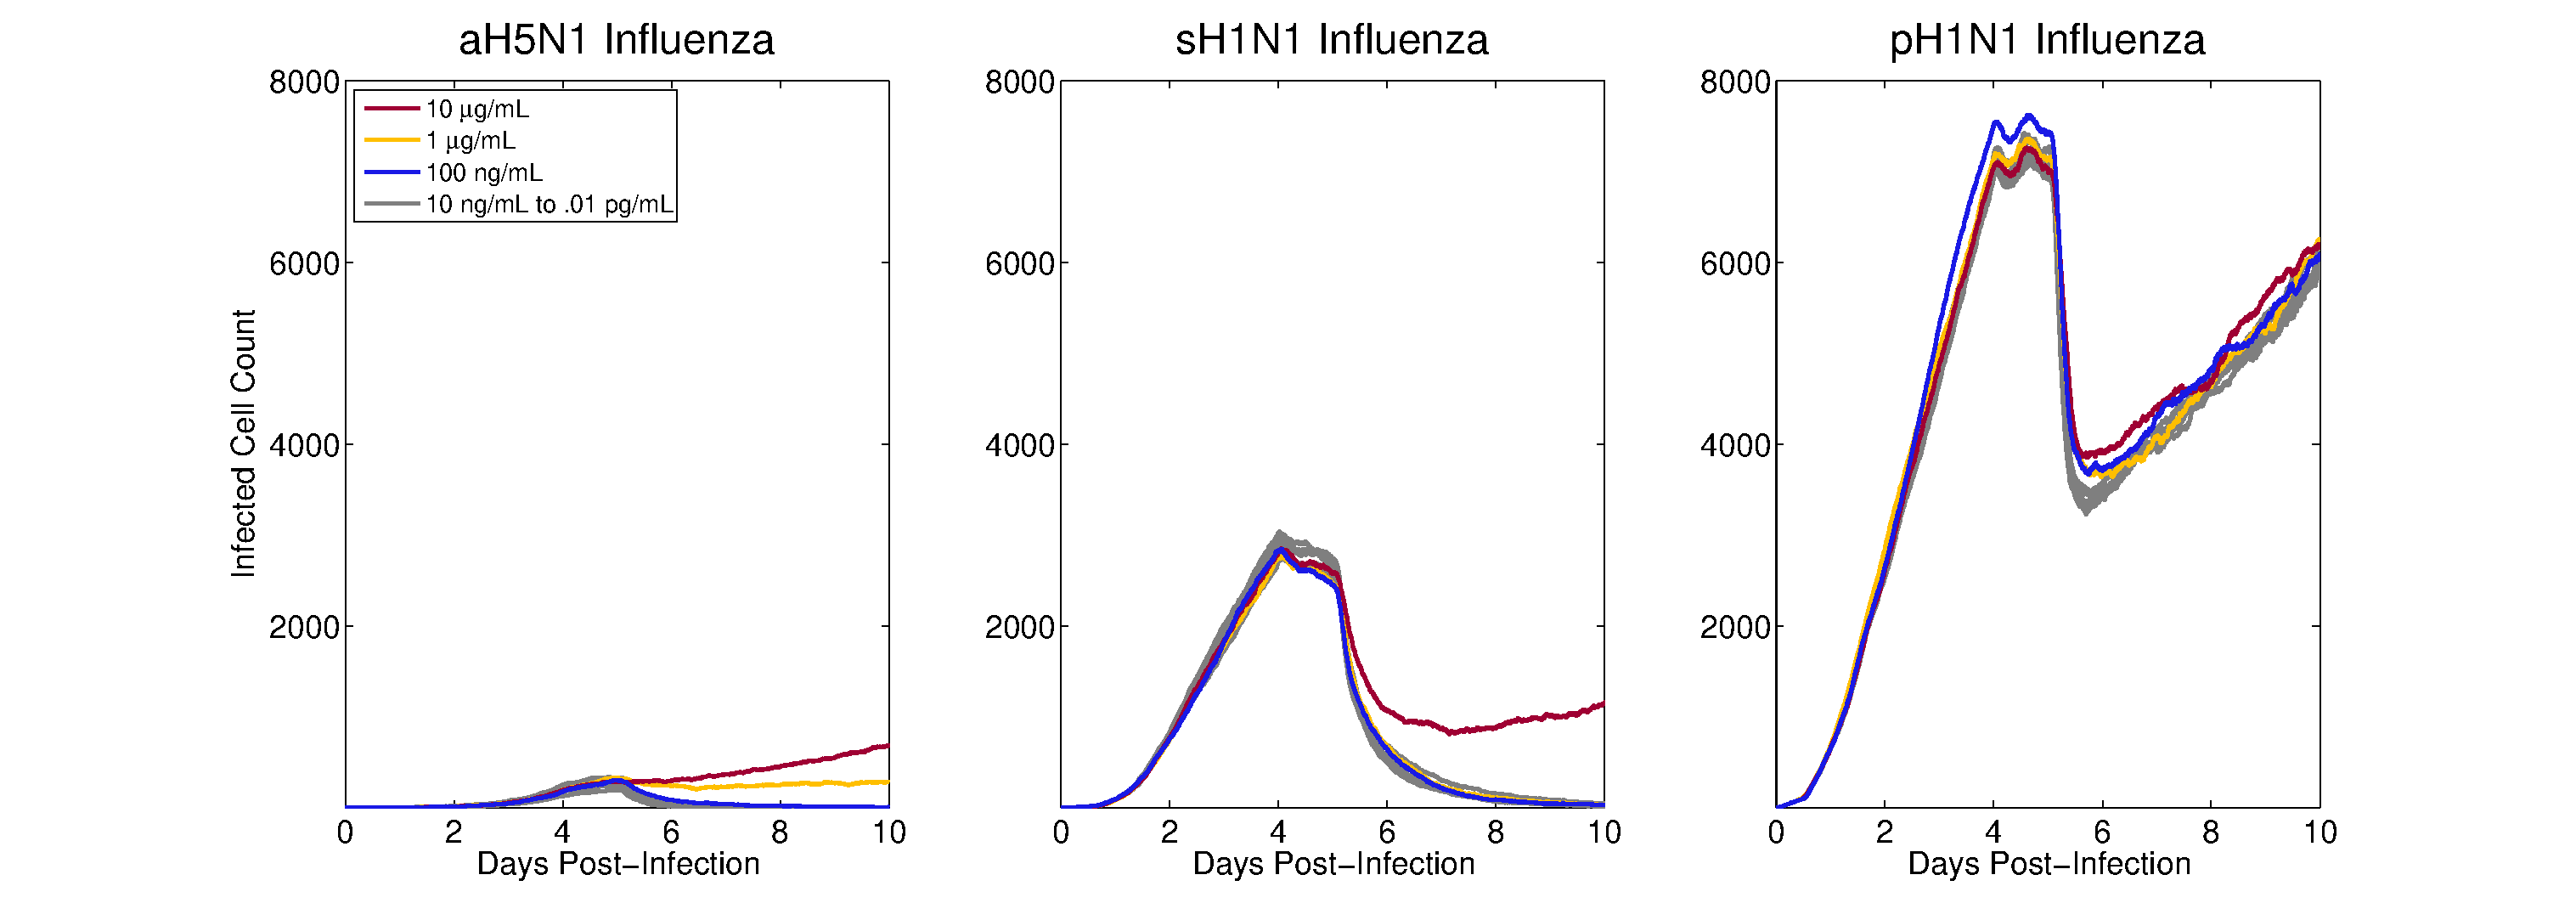
\includegraphics[width=\textwidth]{Figure_S2}
 \end{center}
\caption{{\bf Varying T cell sensitivity to chemokine.}  H5N1 model results use RANTES  only, and sH1N1 and pH1N1 use both IP-10 and RANTES. Total number of incubating, secreting and apoptotic cells are plotted for each infection.  The sensitivity value specifies the minimum level of chemokine concentration required for T cells to detect it. } 
 \label{fig:sensitivity}
\end{figure}


\begin{figure}[ht!]
\begin{center}
	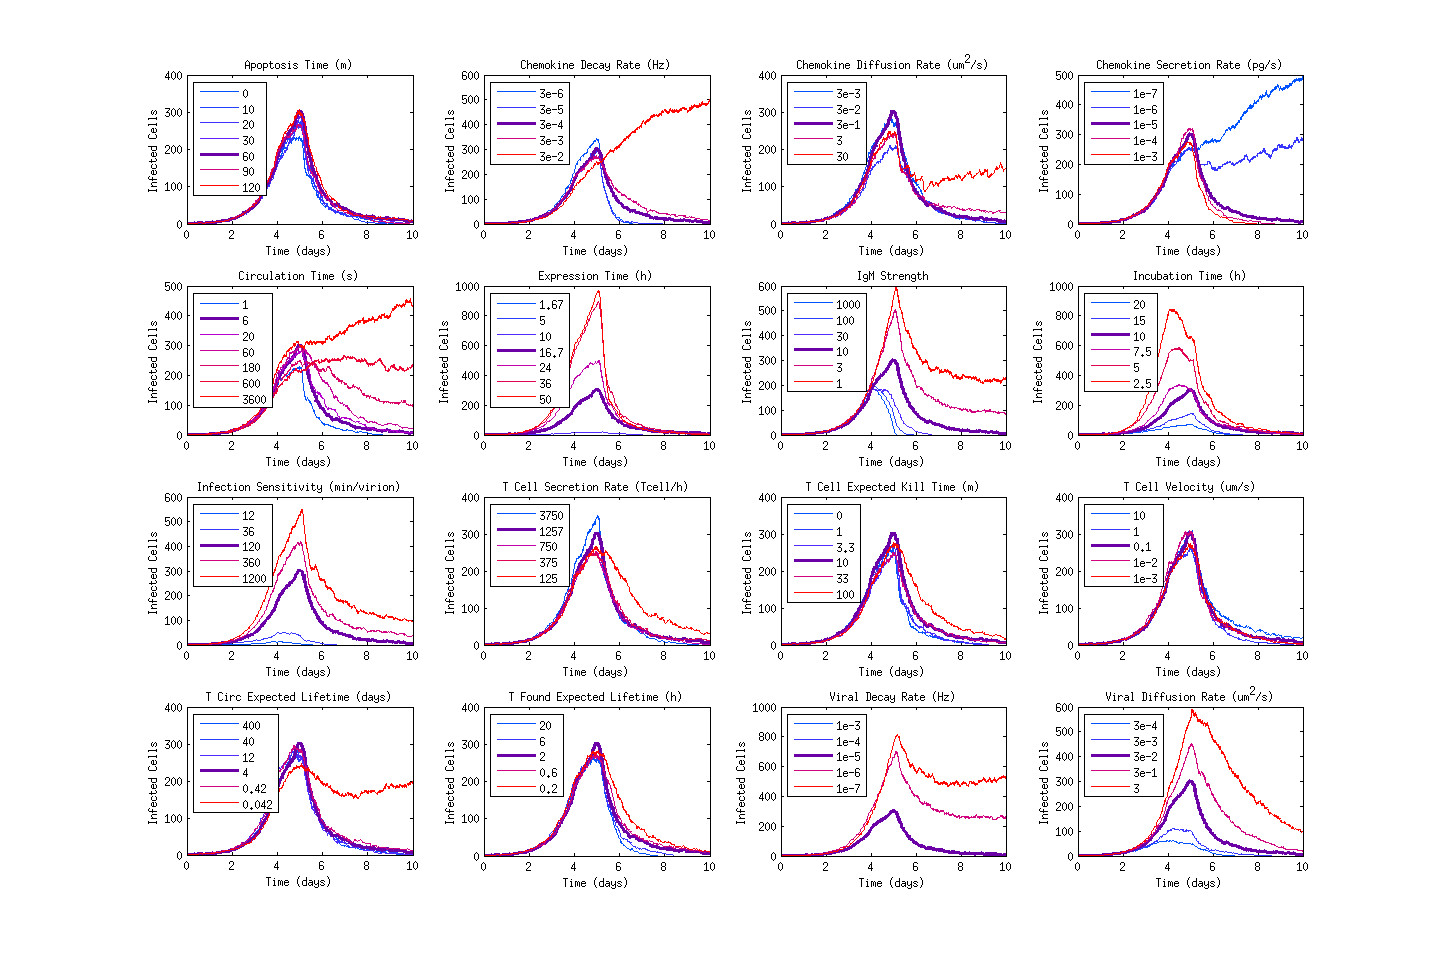
\includegraphics[width=\textwidth]{Figure_S3}
	\caption{\textbf{Effects of different chemokine combinations.}  A) aH5N1 does not stimulate an IP-10 response.  B-C) sH1N1 and pH1N1 show no significant difference between IP-10 alone versus IP-10 and RANTES combined.}
	\label{fig:chemokine}
\end{center}
\end{figure}

\pagebreak
\begin{landscape}

\begin{figure}[ht!]
\begin{center}
	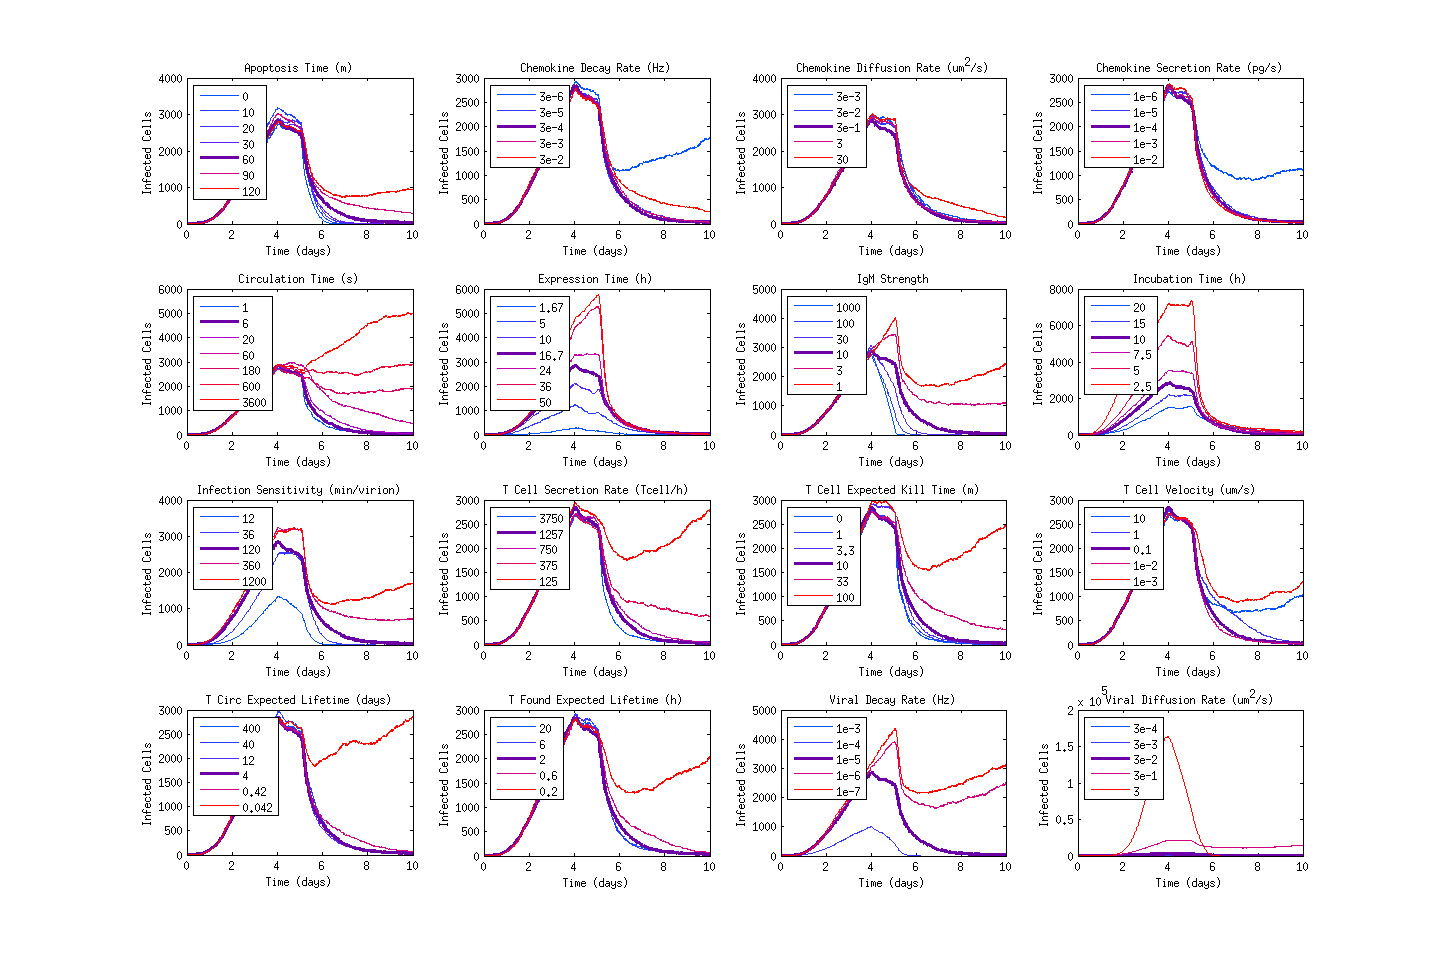
\includegraphics[width=9in]{Figure_S4}
	\caption{\textbf{aH5N1 sensitivity analysis.} The sensitivity analysis results for 16 parameters applied to the aH5N1 model simulation.  In each subgraph, the thicker purple line shows the results of the model using the default parameter value.}
	\label{fig:asensitivity}
\end{center}
\end{figure}

\begin{figure}[ht!]
\begin{center}
	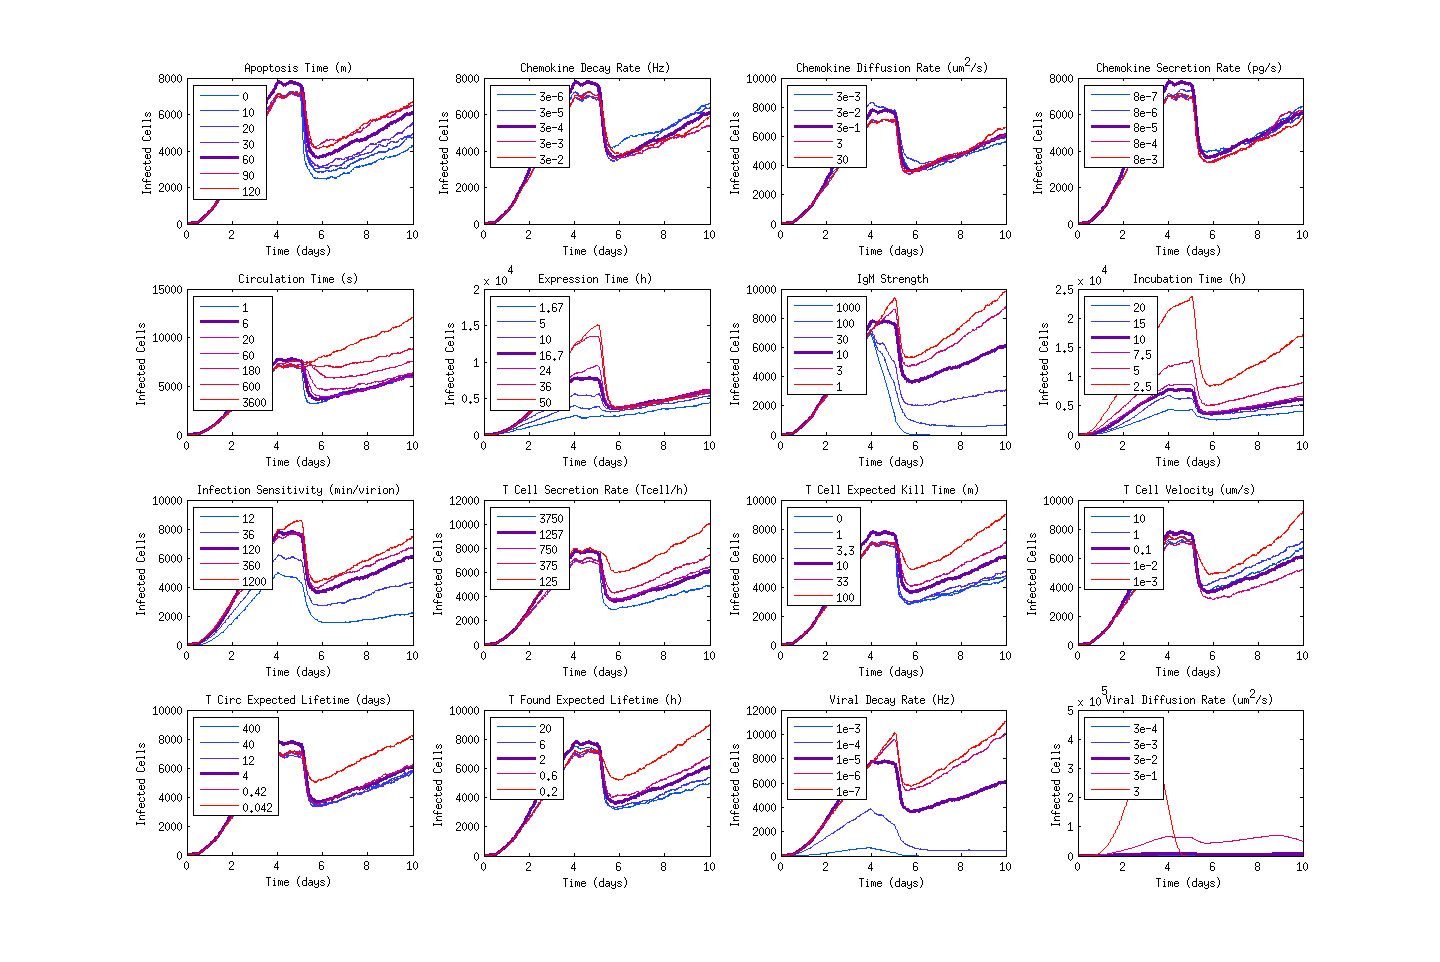
\includegraphics[width=9in]{Figure_S5}
	\caption{\textbf{sH1N1 sensitivity analysis.} The sensitivity analysis results for 16 parameters applied to the sH1N1 model simulation.  In each subgraph, the thicker purple line shows the results of the model using the default parameter value.  The divergence between Apoptosis Time values of 90m and 120m (upper-left plot) highlights an important threshold of infection control.}
	\label{fig:ssensitivity}
\end{center}
\end{figure}

\begin{figure}[ht!]
\begin{center}
	\includegraphics[width=9in]{Figure_S6}
	\caption{\textbf{pH1N1 sensitivity analysis.} The sensitivity analysis results for 16 parameters applied to the pH1N1 model simulation.  In each subgraph, the thicker purple line shows the results of the model using the default parameter value.}
	\label{fig:psensitivity}
\end{center}
\end{figure}

\begin{figure}[ht!]
\begin{center}
	\includegraphics[width=9in]{Figure_S7}
	\caption{\textbf{PRCC sensitivity analysis.} PRCC analysis generated Spearman correlation coefficients ($\rho$) and significance values ($p$) over 1441 time points.  Plots show values of $\rho$ vs. time for each parameter tested.  Dark blue indicates significance levels at $p < 0.01$.  Gold indicates significance of $p < 0.05$.  Light gray indicates $p \geq 0.05$.  Six parameters show significant effect over the time period where they were relevant to model dynamics: infected cell expression time, viral response to IgM, viral infectivity, T cell expected lifetime at the FOI, viral decay rate, and the viral diffusion rate.}
	\label{fig:prcc}
\end{center}
\end{figure}

\end{landscape}

\begin{figure}[ht!]
\begin{center}
	\includegraphics[width=\textwidth]{Figure_S8}
	\caption{\textbf{PRCC sensitivity analysis for the viral secretion rate.} Similar to Figure S6, PRCC analysis generated Spearman correlation coefficients ($\rho$) and significance values ($p$) over 1441 time points.  Plot shows the values of $\rho$ vs. time for the viral secretion rate.  Dark blue indicates significance levels at $p < 0.01$.  Gold indicates significance of $p < 0.05$.  Light gray indicates $p \geq 0.05$.  Viral secretion shows significant effect on model output.  The decline of $\rho$ over time reflects the early death of every modeled target cell (Figure~\ref{fig:exhaustive})).}
	\label{fig:vsec}
\end{center}
\end{figure}

\begin{figure}[ht!]
\begin{center}
	\includegraphics[width=\textwidth]{Figure_S9}
	\caption{\textbf{Exhaustive Growth:} Certain parameter sets generated by Latin hypercube sampling caused rapid uncontrolled infection growth (Samples 1-3).  This resulted in the early death of every modeled target cell (saturation at day 1) and the inevitable decline of the infection size to zero.  A larger, unbounded model environment would show unconstrained growth.  This effect explains the decline of the $\rho$ value of several viral parameters to or past zero over time in Figures \ref{fig:prcc} and \ref{fig:vsec}.}
	\label{fig:exhaustive}
\end{center}
\end{figure}




%\begin{figure}[ht!]
%\begin{center}
%	\includegraphics[width=\textwidth]{Figure_SX}
%	\caption{\textbf{pH1N1 sensitivity analysis.} Model results and fits of the viral effectiveness rate, $E$.}
%	\label{fig:effectiveness}
%\end{center}
%\end{figure}


%\begin{figure}[ht!]
%\begin{center}
%	\includegraphics[width=\textwidth]{Figure_SX}
%	\caption{\drew{\textbf{Effects of different T cell speeds.}  With the exception of sH1N1, T cell speeds show a small effect during the early phase of the T cell response.  After a time of approximately two days, the infection dynamics converge to a similar rate of growth across all speed values.}}
%	\label{fig:speed}
%\end{center}
%\end{figure}

\setcounter{figure}{0}
\renewcommand{\figurename}{Video}


\begin{figure}[ht!]
\caption{The first of three overlaid videos of a representative seasonal H1N1 infection.  This video spans the 10 day infection and shows the cells as they transition from healthy to infected to dead.  T cells show half way through the simulation.  Healthy cells are gray, virus-incubating cells are yellow, virus-secreting cells are orange, apoptotic cells are red, and T cells are green.} 
 \label{video:cell_view}
\end{figure}

\begin{figure}[ht!]
\caption{The second of three overlaid videos of a representative seasonal H1N1 infection.  This video spans the 10 day infection and shows the virus concentration.  Notice the volatility when T cells arrive halfway through the simulation.  Virus concentration ranges from 1e-13 mols/mL (white) to 1e-27 mols/mL (black).  Refer to Figure 5 for the detailed legend. } 
 \label{video:virus_view}
\end{figure}

\begin{figure}[ht!]
\caption{The third of three overlaid videos of a representative seasonal H1N1 infection.  This video spans the 10 day infection and shows the chemokine concentration.  Notice the volatility when T cells arrive halfway through the simulation.  Chemokine concentration ranges from 1e8 ng/mL (white) to 1e-6 ng/mL (black).  Refer to Figure 5 for the detailed legend. } 
 \label{video:chemokine_view}
\end{figure}

\begin{figure}[ht!]
\caption{A closer look at the 2009 pandemic simulation.  This video shows the infection from day 6 to day 7 with each frame spanning 1 simulated minute.  Healthy cells are gray, virus-incubating cells are yellow, virus-secreting cells are orange, apoptotic cells are red, and T cells are green.  Note the high proportion of virus-secreting cells (orange) early on.  As time passes, secreting cells are gradually contained to the point where they become very sparse.  T cell clumping often prevents the T cells from quick discovery of new secreting cells.}
\end{figure}

\pagebreak

\section*{Tables}

%\begin{table}[!ht]
%\caption{
%\bf{Table title}}
%\begin{tabular}{|c|c|c|}
%table information
%\end{tabular}
%\begin{flushleft}Table caption
%\end{flushleft}
%\label{tab:label}
% \end{table}

\renewcommand{\thetable}{S\arabic{table}}

\begin{table}[!ht]
\begin{center}
\begin{tabular}{| r r r | c | r r r | c | r r r |}
  \multicolumn{3}{c}{aH5N1} & \multicolumn{1}{c}{} & \multicolumn{3}{c}{sH1N1} & \multicolumn{1}{c}{} & \multicolumn{3}{c}{pH1N1}\\
  \cline{1-3} \cline{5-7} \cline{9-11}
  Time & CXCL10 & CCL5 & & Time & CXCL10 & CCL5 & & Time & CXCL10 & CCL5 \\
   \multicolumn{1}{|c}{\footnotesize{$hours$}} & \multicolumn{1}{c}{\footnotesize{$pg/mL$}} & \multicolumn{1}{c|}{\footnotesize{$pg/mL$}} & & \multicolumn{1}{c}{\footnotesize{$hours$}} & \multicolumn{1}{c}{\footnotesize{$pg/mL$}} & \multicolumn{1}{c|}{\footnotesize{$pg/mL$}} & & \multicolumn{1}{c}{\footnotesize{$hours$}} & \multicolumn{1}{c}{\footnotesize{$pg/mL$}} & \multicolumn{1}{c|}{\footnotesize{$pg/mL$}}\\
  \cline{1-3} \cline{5-7} \cline{9-11}
  0 & 440 & 1 & & 0 & 94 & 62 & & 0 & 179 & 45  \\
  2 & 391 & 0 & & 2 & 24 & 45 & & 12 & 1,835 & 55 \\
  8 & 1,723 & 1 & & 8 & 87 & 50 & & 16 & 1,349 & 46 \\
  12 & 3,462 & 1 & & 10 & 296 & 57 & & 20 & 23,458 & 150 \\
  16 & 4,618 & 2 & & 16 & 770 & 87 & & 24 & 12,073 & 93 \\
  20 & 6,807 & 6 & & 20 & 3,048 & 134 & & 32 & 30,700 & 380 \\
  24 & 8,164 & 16 & & 24 & 3,901 & 151 & & 48 & 19,814 & 1,224  \\
  30 & $>$ 8,500 & 68 & & 28 & 8,261 & 150 &  &  &  &  \\
  38 & $>$ 8,500 & 239 & & 32 & 12,935 & 245 &  &  &  &  \\
  48 & $>$ 8,500 & 655 & & 38 & 26,970 & 780 &  &  &  &  \\
  72 & $>$ 8,500 & 415 & & 42 & 24,120 & 695 &  &  &  &  \\
  & & & & 72 & 21,441 & 1,665 &  &  &  &  \\
    \cline{1-3} \cline{5-7} \cline{9-11}
\end{tabular}
\caption{\textbf{Empirical cytokine titers for three strains of influenza.}  Measured CXCL10 (IP-10) and CCL5 (RANTES) shown in pg/mL for three strains of influenza: Avian H5N1, Seasonal sH1N1, and Pandemic pH1N1.  sH1N1 IP-10 secretion exceeded measurement accuracy above 8500 pg/mL.  Human bronchial epithelial cells were infected at an MOI of 0.01 (10,000 virions) with one of the three strains of influenza.  Basal media for chemokine secretion was collected at the given time intervals post infection.  Chemokine levels were measured using 30 $\mu$L aliots for a panel of 17 chemokines and cytokines (not shown).}
\label{tab:data}
\end{center}
\end{table}

\begin{table}[!ht]
\begin{center}
\begin{tabular}{|  l  l  l  |}
  \hline
  Population & Description & Initial Value\\
  \hline
  $T$ & Healthy target epithelial cells & 1,000,000 \\
  $I_1$ & Virus-incubating cells & 0 \\
  $I_2$ & Virus-secreting cells & 0 \\
  $V$ & Free virus particles & 10,000 \\
  $F$ & Interferon quantity & 0 \\
  $C$ & Chemokine quantity (ng/mL) & 0 \\
  \hline
  \hline
  Parameter & Description & Value \\
  \hline
  $\beta$ & Viral infection rates &  \\
    & \hspace{2em} Avian & 5.3e-7 (PFU$\cdot$h)$^{-1}$ \\
    & \hspace{2em} Seasonal & 6.1e-7 (PFU$\cdot$h)$^{-1}$ \\
    & \hspace{2em} Pandemic &  2.7e-6 (PFU$\cdot$h)$^{-1}$\\
  $p$ & Viral production rates & \\
    & \hspace{2em} Avian & 0.20 (PFU/h) \\
    & \hspace{2em} Seasonal & 1.4 (PFU/h) \\
    & \hspace{2em} Pandemic & 18.3 (PFU/h) \\
  $e$ & Interferon strengths & \\
    & \hspace{2em} Avian & 1.0e-8 \\
    & \hspace{2em} Seasonal & 1.6e-6 \\
    & \hspace{2em} Pandemic & 3.4e-3 \\
  $\tau_2$ & Interferon production delays &  \\
    & \hspace{2em} Avian & 21.5 (h) \\
    & \hspace{2em} Seasonal & 23.6 (h) \\
    & \hspace{2em} Pandemic & 21.0 (h) \\
  $\delta$ & Virus-secreting cell decay rate & 0.6 (h$^{-1}$) \\
  $d$ & Chemokine decay rate & 1.386 (h$^{-1}$) \\
  $\tau_1$ & Viral incubation time & 10 (h) \\
  $\tau_3$ & Chemokine production delays & \\
    & \hspace{2em} IP-10 & 8 (h)\\
    & \hspace{2em} RANTES & 16 (h)\\
  \hline
\end{tabular}
\caption{\textbf{Parameters for Preliminary Model 1 (Equation 1)}.  All parameters and populations are taken from \citep{Mitchell2011} except for $C$, $d$, and $\tau_3$.  The value chosen for $d$ corresponds to a 30 minute half-life and values for $\tau_3$ were set from the observed chemokine data (Fig.~\ref{fig:data}).  Interferon ($F$) is an abstracted unitless quantity and thus $e$ is a unitless multiplier.}
\label{tab:dde}
\end{center}
\end{table}


\begin{table}[!ht]
\begin{center}
\begin{tabular}{| c | c | c |}
  \hline
  Strain & Chemokine & RMSE \\
  \hline
  \multirow{2}{*}{aH5N1} & RANTES & 166 \\
  & IP-10 & 7,950 \\
  \hline
  \multirow{2}{*}{sH1N1} & RANTES & 90 \\
  & IP-10 & 2,732 \\
  \hline
  \multirow{2}{*}{pH1N1} & RANTES & 2,671  \\
  & IP-10 & 64,342 \\
  \hline
\end{tabular}
\caption{\textbf{Root mean squared error of Preliminary Model 1 fits.}  Preliminary Model 1 (Eq. 1) was fit to experimental data (Table~\ref{tab:data}) using a genetic algorithm as described in the main paper.  The resulting model fits can be seen in Figure~\ref{fig:fits}.}
\label{tab:rmse}
\end{center}
\end{table}


\begin{table}[!ht]
\begin{center}
\begin{tabular}{ | c | c | c |}
  \hline                        
  Paramter & Value & Source \\
  \hline
  T(0) & $1e6$ & \citep{Mitchell2011} \\
  V(0) &  $1e4$ & \citep{Mitchell2011} \\
  $r_{cell}$ &  $5 \mu m$ & \citep{Miao2010a} \\
  $t_{rc}$ & $6s$ & \citep{Peters1983} \\
  $k_e$ & $6.4e-5/cell/day$ & \citep{Miao2010a} \\
  $\beta$ & $4.8e-7/cell/PFU$ & \citep{Mitchell2011} \\
  $p$ & $0.18 PFU/h$ & \citep{Mitchell2011} \\
  $\delta$ & $16.7 hours$ & \citep{Mitchell2011} \\
  $a$ & $67.7$ & ABM fits \\
  $b$ & $433.5$ & ABM fits \\
  \hline  
\end{tabular}
\begin{tabular}{| c | c |}
  \hline
  I & C \\
  \hline
  4 & 329 \\
  58 & 997 \\
  816 & 2550 \\
  3,264 & 4,410 \\
  10,050 & 8,069 \\
  \hline
\end{tabular}
\caption{\textbf{Parameters for Preliminary Model 2 (Equation 2).}  Values are chosen to match the equations borrowed from both \citep{Mitchell2011} and \citep{Miao2010a}.  Values \textit{a} and \textit{b} were fit to multiple runs of a simplified CyCells ABM using the linear model $C = a\sqrt{I}+b$ with a resulting $R^2 = 0.997$, $P < 0.01$.}
\label{tab:supplement}
\end{center}
\end{table}


\begin{table}[!ht]
\centering
\begin{tabular}{| c | l | c | l |}
  \hline                        
  Category & Parameter & Units & Distribution \\
  \hline
  \multirow{3}{*}{Chemokine} & Chemokine Decay Rate & \textit{Hz} &  LN(-3.4, 1.0) \\
  & Chemokine Diffusion Rate & \textit{$\mu$m$^2$/s} & LN(-0.5, 1.0) \\
  & Chemokine Secretion Rate & $(pg/s\cdot cell)$ & LN(-3.7, 0.1) \\
  \hline
  \multirow{6}{*}{T Cell} & Circulation Time & \textit{seconds} & LN(-.75, 0.5)\\
  & T Cell Kill Rate & \textit{min} & LN(1.0, 0.5) \\
  & T Cell Speed & \textit{$\mu$m/min} & LN(-.75, 1), \\
  & T Cell Age in Blood & \textit{days} & LN(0.6, 1.0) \\
  & T Cell Age at FOI& \textit{min} & LN(2.1, 0.5) \\
  & T Cell Production Rate & \textit{cells/h} & LN(3.1, 0.15) \\
  \hline
  \multirow{3}{*}{Delay} & Apoptosis Time & \textit{hours} & U(0.0, 2.0) \\
  & Expression Time & \textit{min} & LN(3.0, 0.15) \\
  & Incubation Time & \textit{hours} & LN(-1.0, 0.15) \\
  \hline 
  \multirow{4}{*}{Virus} & Viral Response to IgM & | & LN(1.0, 0.5) \\
  & Infectivity & \textit{min/virion} & LN(2.1, 0.5) \\
  & Viral Decay Rate &  \textit{day$^{-1}$} & LN(0, 1.0) \\
  & Viral Diffusion Rate & \textit{$\mu$m$^2$/s} & LN(-1.5, 1.0) \\
  & Viral Secretion & $(PFU/s\cdot cell)$ & LN(-3.4, 0.3) \\
  \hline  
\end{tabular}
\caption{\textbf{Latin hypercube sampling distributions.}  LHS was used to generate sample points containing each of the 16 parameters from Table \ref{tab:sensitivity}, plus the sH1N1 viral secretion rate.  Parameters were sampled over biologically plausible ranges listed here for use in PRCC analysis.  LN signifies a log-normal distribution.  Values were sampled from a regular normal distribution with the listed parameters and then transformed to linear space from $log_{10}$ space.  U signifies a uniform distribution.}
\label{tab:lhs}
\end{table}
 

\begin{table}[!ht]
\centering
\begin{tabular}{ | c  r | c  c | }
  \hline                        
  \multicolumn{2}{|c|}{\multirow{2}{*}{Strain}} & Slope & Intercept \\
  \multicolumn{2}{|c|}{} & \footnotesize{$(PFU/s)$}  & \footnotesize{$(PFU)$} \\
  \hline
  \multirow{2}{*}{Avian H5N1} & I(t) & 5.86e-8 & -0.0133 \\
   & D(t) &  1.03e-7 & -0.0223 \\ 
   \hline
  \multirow{2}{*}{Seasonal H1N1} & I(t) & 3.25e-7 &  0.0225\\
  & D(t) &  6.93e-6 & 0.0439 \\
   \hline
  \multirow{2}{*}{Pandemic H1N1} & I(t) & 8.79e-7 & 0.093 \\
   & D(t) & 2.71e-4 & 5.28 \\
  \hline
  \hline
  \multicolumn{2}{|c|}{Strain} & Avg. $E(t)$ & Estimated $R_0$ \\
  \hline
  \multicolumn{2}{|c|}{Avian H5N1} & 0.355 & 1.16 \\
  \multicolumn{2}{|c|}{Seasonal H1N1} & 0.049 & 1.11 \\
  \multicolumn{2}{|c|}{Pandemic H1N1} & 0.0037 & 1.12 \\
  \hline
\end{tabular}
\caption{\textbf{Linear fits to model runs for $I(t)$ and $D(t)$ across all three strains.}  Every parameter was significant at the $p < 0.05$ level.  $E(t)$ is estimated to be $I(t) / [I(t) + D(t)]$.  $E(t)$ does not vary by more than 10\% from day 5 to day 10, thus the average of each is calculated and used to estimate $R_0$ for all three strains in the absence of a T cell response.}
\label{tab:effectiveness}
\end{table}
 

%\begin{table}[!ht]
%\begin{center}
%\begin{tabular}{ | c | c | }
%  \hline                        
%  Assumption & Description \\
%  \hline
%  2D hexagonal layout & The lung can be stretched flat.  T cells travel on the cellular surface. \\
%  Even blood flow to all capillaries & We assume that there is negligible increased blood flow to the infected region. \\
%  Rapid T cell circulation & Activated T cells in circulation do not spend time in new lymph nodes as they circulate. \\
%  T cell speed & T cells move at a rate of XXX in the absence of chemokine and XXXX once it detects chemokine. \\
%  T cell search time & T cells search in the lung for 6 minutes before they recirculate. \\
%  \hline  
%\end{tabular}
%\caption{Supplemental model parameters.  Most values are chosen to match the equations borrowed from both \citep{Mitchell2011} and \citep{Miao2010a}.  Values \textit{a} and \textit{b} were fit to multiple runs of a simplified CyCells ABM.}
%\label{table:assumptions}
%\end{center}
%\end{table}

\end{document}
